\documentclass[12pt]{article}
\usepackage[margin=1in]{geometry}
\usepackage[utf8]{inputenc}
\usepackage{setspace}
\usepackage{titlesec}
\usepackage{amsmath,amsthm,amsfonts,mathtools,color,amssymb}
\usepackage{tikz}
\usepackage{mathrsfs}
\usepackage{biblatex}

\titlespacing*{\section}
{0pt}{1em}{1em}
\titlespacing*{\subsection}
{0pt}{.5em}{.5em}
\titlespacing*{\subsubsection}
{0pt}{.25em}{.25em}

\title{Masters Project Report}
\author{Emily Palmer}
\date{Spring 2021}

\addbibresource{bib.bib}
\doublespacing

\begin{document}

\maketitle

\begin{abstract}
  The Microbiome Taxonomic Longitudinal Correlation, a recent model for microbiome association studies, was explored in detail and code was developed for application in general datasets beyond the case study provided in the initial paper. Applications of this method provided computational challenges when the scale of the data is beyond a small number of selected OTUs.
\end{abstract}

% Several aspects of the method to more general data were developed for use beyond the case study provided in the initial paper.
% Application of a recent method for microbiome association studies to larger datasets provided computational challenges.
% \tableofcontents



\section{Introduction}

\subsection{Microbiome data}
The human gut contains millions of microbes. Genomic research on microbiome sequencing data has provided numerous insights to human health. Studies have associated the human gut microbiome to irritable bowel syndrome, inflammatory bowel disease, cancers, diabetes, and obesity, and shown the existence of bi-directional interactions  between the gut and the central nervous system \cite{kinross2008human, mayer2015gut}. These studies show the human microbiome to be a research rich and important area of focus.
% Characteristics of these data make these data difficult to analyze using standard statistical methods, so there is also needed work to develop or alter the statistical approaches used for this type of data.


Microbiome data commonly arises from 16S ribosomal ribonucleic acid RNA (16s rRna) sequencing studies. This gene is a useful marker for microbe identification.  Microbiome sequencing data commonly consists of the count of reads on operational taxonomic units (OTUs) for each sample. Operational taxonomic units refer to the bins in which sequences are grouped, and are frequently mapped back to taxonomic labels from existing libraries. Methods for microbiome analysis can either be focused on a single OTU or multiple OTUs simultaneously.

% Microbiome sample can be collected from fecal samples, but oral, skin, vaginal, etc are also common areas (CITE).

There are several aspects common to microbiome OTU data that present obstacles to analysis using standard statistical approaches. The number of OTUs is often very large compared to the sample size. The value of the count for a given OTU is dependent on the sampling depth for the given sample (the sum of all OTUs across the sample). This sampling depth is not originally constant across samples, so  normalization is necessary before counts can be compared across samples. This can be done by rarifying, or randomly sampling OTUs to standardize the sampling depth across samples. Often, OTU counts are converted into a proportion to represent the relative abundance of that OTU in the sample.

Additionally, OTU data is very sparse, with many samples having zero counts across multiple OTUs. Thus microbiome data contains excessive zeros, which much be accounted for in the analysis. Common adjustments are either to use models based on zero inflated distributions, or two-part models that separately model the presence of an OTU and the abundance (or relative abundance) of present OTUs.


% The library size of different samples can vary.
 % that violate the assumptions of common statistical tests and regression models.
% Frequently, the sampling depth (FINISH) is not consistent across samples. One technique to adjust for this is rarifying (CITE, FINISH)

% The count for a given OTU does not necessarily represent the overall count. In other words, these counts represent relative abundance, not absolute abundance, and the counts between samples cannot be directly compared as they are constrained by the overall sampling depth, which is not consistent across samples. OTU data is thus compositional in nature. Often, OTU counts are converted into a proportion to represent the relative abundance of that OTU in the sample.


% The microbiome is not static. Longitudinal
%
% SECTION ON LONGITUDINAL STUDIES, define longitudinal data


\subsubsection{Taxonomic tree for OTUs}

Two types of trees can arise in microbial studies: phylogenetic trees and taxonomic trees. Phylogenetic trees estimate the evolutionary history between organisms by splitting of a tree to represent shared ancestors. Taxonomic trees represent the hierarchy of shared labels of different classified taxa levels: Kingdom, Phylum, Class, Order, Family, Genus, and Species. Ideally, these two trees should be equivalent, but this requires explicit naming and organizing of each bacterial species, which is an imposing and incomplete task. The taxonomic labeling system is coarse for microbial species, and new discoveries and changing naming systems will change its structure \cite{washburne2018methods}. This project will focus on taxonomic trees.

% (FIND ANOTHER SOURCE )
When association studies are performed using multiple OTUs, it can be reasonable to use prior knowledge on the given evolutionary or hierarchical organizational relationship between multiple OTUs. Potentially, evolutionally relationships might correspond to similar relationships between the OTU expression, and chosen covariates. If a certain OTU is found to be associated with a covariate, we might expect another OTU that is close on the taxonomic tree to   also be associated with a covariate, and associated in a similar way. Broadly, we want to use the knowledge of the placement of a given OTU on the taxonomic tree to provide insight into correlations that exist between different read counts present in samples. Hopefully this correlation can be helpful in modeling overall association with predictors of interest.





\subsection{Generalized Estimating Equations}

Generalized Estimating Equations (GEEs) were introduced to extend generalized linear models to analysis of longitudinal data \cite{liang1986longitudinal}. They are a useful tool for analyzing correlated data, such as can arise from longitudinal data, but also more generally for data with correlations from any sort of repeated measure. GEEs estimate population average effects by assuming a within cluster correlation structure.


% While initially aimed for correlations arising from longitudinal data, GEEs can be useful for data with any sort of correlations, longitudinal, repeated measure, etc (FINISH).

% Generalized Estimating Equations (GEEs), introduced to extend generalized linear models to longitudinal data,  are a useful tool for analyzing correlated data, such as those that arise from longitudinal data. GEEs were introduced to extend generalized linear models to longitudinal data \cite{liang1986longitudinal}. While initially aimed for correlations arising from longitudinal data, GEEs can be useful for data with any sort of correlations, longitudinal, repeated measure, etc (FINISH).


First, we introduce some notation. A cluster $\mathbf{y}_k$ is the collection of points from repeated measures $\mathbf{y}_k = (y_{k,1}, \ldots , y_{k,n_j})$ taken from a subject, or individual, $k$ where $k = 1, \ldots , K$ represents the index of clusters/individual, and $j = 1, \ldots , n_k$ represent the different repeated measures taken, for instance, values on different  time points, sample sites, or OTU measurements, or any other given repeated measurement taken on a cluster.
The concept of a cluster will depend on the data setting, for instance we could even consider a family as the cluster designation. For instance, consider the response variable for a family $k$, measured on two family members (perhaps twins), on 2 days and 2 OTU measurements. Then $\mathbf{y}_k = (y_{k, f_1,t_1,1}, y_{k, f_1,t_1,2}, y_{k, f_1,t_2,1}, y_{k, f_1,t_1,2},y_{k, f_2,t_1,1}, y_{k, f_2,t_1,2}, y_{k, f_2,t_2,1}, y_{k, f_2,t_1,2})$, where $f_i$ represents the family index, $t_i$, represents the time index, and $o_i$ represents the OTU index.
% For instance, if individual $\mathbf{y}_1$ was sampled on three different days, $\mathbf{y}_1 = (y_{1,1}, y_{1,2}, y_{1,3})$ represent the response value for individual $1$ on the 3 different days. Alternatively, this could represent if we sampled values of 3 different OTUs, instead of 3 different days.

We additionally have a $p \times 1$ vector of covariates $x_{kj}$ measured for the $j$th value on each cluster $k$.The model of the GEE links the mean of the responses to the covariates through the following regression equation.
$$g(\mu_{kj}) = \mathbf{x}_{kj}^T\boldsymbol \beta$$
where $E(\mathbf{y_{kj}} = \mu_{kj}$ and $g(\cdot)$ is a known link function. The variance of the responses is $\text{Var}(Y_{kj}) = \phi a_{jk}$, where $\phi$ is the dispersion parameter and $a_{jk}$ is a known variance function determined by the distribution of the data. Let $R_k(\alpha)$ be the specified working correlation matrix, which is specified by the distinct values of $\alpha$, that describes the assumed within-cluster correlation structure. Define
$$V_k = \phi A_k^{-1/2} R_{i(\alpha)}A_i^{1/2}$$ as the working covariance matrix of $Y_k$, where $A_k$ is the diagonal matrix consisting of the values of $a_{jk}$. Then, $\hat{\boldsymbol\beta}$ is the solution to the following Generalized Estimating Equation.
$$\sum_{k=1}^K \frac{\partial  \mu_k^T }{\partial \beta } V_{k}^{-1} (Y_k - \mu_k) = 0 $$
The above equation depends on the values of $\alpha$ and $\phi$, so these must additionally be estimated. The solution to the above equation is found using an iterative formula that switches between estimating $\hat\beta$ using given fixed $\hat \alpha, \hat \phi$ and estimating $\alpha,  \phi$ using given fixed $\beta$. GEEs work without specifying the joint distribution of observations, similarly to quasi-likelihood approaches.

One useful characteristic of GEEs is that the parameter estimation of $\beta$ is consistent, even if the working correlation matrix is misspecified. The estimate $\hat{\boldsymbol\beta}$ is asymptotically normally distributed with mean $\boldsymbol\beta$ and variance
$$ \big(\sum_{k=1}^K  \frac{\partial  \mu_k^T }{\partial \beta } V_k^{-1} \frac{\partial  \mu_k }{\partial \beta^T } \big)^{-1} \bigg(\sum_{k=1}^K  \frac{\partial  \mu_k^T }{\partial \beta } V_k^{-1}\text{COV}(Y_i)V_{k}^{-1}  \frac{\partial  \mu_k }{\partial \beta^T } \bigg)\big(\sum_{k=1}^K  \frac{\partial  \mu_k^T }{\partial \beta } V_k^{-1} \frac{\partial  \mu_k }{\partial \beta^T } \big)^{-1}$$
Where $\text{COV}(Y_k)$ is the true covariance matrix of $\mathbf{y}_k$

If we replace $ \boldsymbol\beta, \phi, \alpha$ and $\text{COV}(Y_k)$ with $\hat\beta, \hat \alpha, \hat \phi$ and $(Y_k - \mu_k)(Y_k- \mu_k)^T$ this gives us the sandwich estimator, a constant estimator for the variance of $\boldsymbol\beta$.


\subsubsection{GEEs in R}

The \texttt{geepack} package\cite{geepack} in R \cite{R} provides a useful way to implement GEEs with a user defined working correlation structure, denoted \texttt{zcor}. The function \texttt{geeglm()} fits a GEE from the specified regression formula, link function, and correlation structure, similarly to the standard \texttt{glm()} function call.

There are four main pre-specified working correlation matrix structures in \texttt{geeglm}: independence, exchangeable, AR1, and unstructured. Specifying a user-defined correlation structure is also possible, although seems much less common in applications than using the pre-defined structures. The format of the user-defined correlation structure \texttt{zcor} is different than the working correlation matrix defined above the GEE framework. The GEE working correlation matrix $R_k(\alpha)$ is a square matrix that has the same dimension as the length of $\mathbf{y}_k$ for the $k$th cluster. In contrast, \texttt{zcor} uses the upper diagonal correlation parameters of the working correlation matrix $r_k = (r_{k, 12}, r_{k,13}, \ldots , r_{k,1n_k}, r_{k,23}, \ldots , r_k{k,n_{k-1}n_k})$ of $R_{k}(\alpha)$ . The \texttt{zcor} $Z_k$ matrix for cluster $k$ comes from $r_k = Z_k \alpha$. The overall \texttt{zcor} matrix comes from combining these matrices $(Z_1^t, \ldots , Z_K^t)^t$. This matrix will have dimension $\sum_{k=1}^K \binom{n_k}{2} \times m$, where $m$ is the length of $\alpha$.



\section{Microbiome Taxonomic Longitudinal Correlation (MTLC) model}

The Microbiome Taxonomic Longitudinal Correlation (MTLC) model was introduced in 2020 by Chen and Xu\cite{chen2020generalized} as a way to estimate correlations between OTUs as well as associations between OTU responses and covariates, that can be used on longitudinal and repeated measure data. Coefficients are estimated using a two part GEE model that uses a correlation structure based on OTU taxonomy and longitudinal and repeated measure correlations.



\subsection{Model Data structure}
Commonly, OTU information is stored in two tables, an OTU table and a metadata table. The rows of the OTU table are the OTU ids, and the columns are the samples. In the metadata table, the rows are samples. Consider a dataset with $K$ individuals;  Each individual has $N$ OTU measurements, and each of these measurements are taken $L$ different repeated measures. In this model, the response is the OTU value (either presence absence, or transformed relative abundance). Both the response, and predictors, must be transformed into a 'long' format.

% The first table contains counts for OTU values, with OTU labels as rows and samples as columns. This table will have overall dimension $N \times M$ The second table contains metadata (predictor) information, with samples as rows and predictor values as columns, having dimension $M \times p$.


% If there are $N$ OTUs recorded, the response is given as $\mathbf{y} = (\mathbf{y}_1, \ldots, \mathbf{y}_K)^t$, where for a given individual/cluster $\mathbf{y}_k = (y_{k,1}, \ldots, y_{k,n_k})$. The vector of covariates for a given $k,j$ has length $p$.

Consider a small example, where there is only one subject, measured at two time points, for two OTUs. The table on the right represents the OTU table, which is then transformed into the form we need for the model.
\begin{singlespace}
$$
\begin{array}{c| c c}
  & S_1,T_1 & S_1,T_2\\
  \hline
  OTU_1 & y_{S_1,T_1,OTU_1} & y_{S1,T2,OTU1}\\
  OTU_2 & y_{S1,T1,OTU2} & y_{S1,T2,OTU2}\\
\end{array}
\qquad \Rightarrow \qquad
\mathbf{y} = \begin{pmatrix}
    y_{S1,T1,OTU1}\\
    y_{S1,T1,OTU2}\\
    y_ {S1,T2,OTU1}\\
    y_{S1,T1,OTU2}
\end{pmatrix} \quad
\mathbf{x} = \begin{pmatrix}
      x_{S1,T1}\\
      x_{S1,T1}\\
      x_{S1,T2}\\
      x_{S1,T2}
\end{pmatrix}
$$
\end{singlespace}
The observations in $\mathbf{y}$ are now not independent. There exist possible correlations between the time points, as well as possible correlations between the OTUs measured. The following sections will explain how these two types of correlations are incorporated into GEE models.

\subsection{Accounting for Correlation}
\subsubsection{Taxa correlation}

Previous studies considering the correlations between OTUs have used a Dirichlet multinomial distribution \cite{la2012hypothesis}. However, this assumes a negative correlation between OTUs, which can be reasonable given the compositional nature of the data,. However, the true correlation structure between OTUs can be positive or negative\cite{mandal2015analysis}, and we want to build models that can account for this flexibility depending on the nature of how given OTUs interact.

In order to model the correlation structure between OTUs, the MTLC model uses the taxonomic information hierarchy of each OTU to specify the OTU correlation aspect of the working correlation matrix used in GEE estimation, denoted $\Gamma$. In order to reduce from an unspecified correlation matrix, where each OTU has a different correlation (which becomes infeasible to model), we impose the assumption that OTUs have the same correlation if the first shared higher level taxa is the same. Determining the unique correlations will depend on the structure of the taxonomic tree. We will then represent the correlation information from the taxonomic tree into a correlation matrix that keeps track of which correlations are the same.

A taxonomic tree can be represented as a list containing counts of how many OTUs belong each subgroup of successive labels. The highest level should contain all $N$ OTUs, and the lowest level should contain $N$ groups, each with $1$ observation. Consider a taxonomic tree that represents the class, order, family, and genus taxonomic labels for five OTUs. The list \texttt{list(5, c(3,2), c(2,1,1,1), c(1,1,1,1,1))} represents the below tree, as the single class contains all 5 OTUs, the first Order group contains 3 OTUs, and the second contains 2, etc.

\begin{singlespace}
$$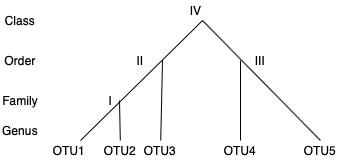
\includegraphics[width = .4\textwidth]{tree.png}
\longrightarrow \Gamma = \begin{pmatrix}
        1 & I & II & IV & IV \\
        I & 1 & II & IV & IV \\
        II & II & 1 & IV & IV \\
        IV & IV & IV & 1 & III \\
        IV & IV & IV & III & 1
  \end{pmatrix}$$
\end{singlespace}

The roman numerals represent the distinct correlations we assume for the working correlation matrix. In this example, correlation $I$ represents OTUs in the same family, but different genus, $II$ and $III$ represent same orders, but different families, and $IV$ represents different orders but the same class.



\subsubsection{Longitudinal and repeated measure correlation}

Additional correlations in the data occur from repeated measures. A common form of repeated measure comes from measurements at different discrete time points. Auto-regressive, Toeplitz, unstructured, exchangeable, and independent are all common correlation structures that can be can be used on longitudinal data. Each of these structures gives a working correlation matrix that indicates the distinct correlation between points. Any of these can be used for longitudinal repeated measures in this model. If there are additional repeated measures in the data besides those from longitudinal measures, the repeated measure working correlation matrix is found by taking all combinations of time points and repeated samples into one repeated measure working correlation matrix. If we have $T$ time points and $S$ different additional repeated measures, the repeated measure working correlation matrix $\Omega$ has dimension $(T \cdot S) \times (T \cdot S ) $

\subsubsection{Integrative correlation matrix }

Specifying the working correlation matrix to use in GEE estimation combines both the taxonomic correlation matrix and repeated measure correlation matrix. The integrative correlation matrix $R$ is a block matrix containing entries $\Omega(\Gamma_{ab})$, where $a,b: 1, \ldots , N$. If we have $N$ different OTUs, and $L$ different repeated measures, the integrative correlation matrix $R$ has dimension $(N \cdot L) \times (N \cdot L)$, where every sub-matrix in $R$ represents the distinct correlations representing the given time/repeated measure/OTU correlation.

For example, if we have data with the OTU structure above, and two time points, which we assume are correlated, the integrative correlation matrix would be

\begin{singlespace}
$$R = \begin{pmatrix}
        1 & 2 & 3 & 5 & 5 &  6 & 7 & 8 & 10 & 10 \\
        2 & 1 & 3 & 5 & 5 & 7 & 6 & 8 & 10 & 10 \\
        3 & 3 & 1 & 5 & 5 & 8 & 8 & 6 & 10 & 10 \\
        5 & 5 & 5 & 1 & 4 & 10 & 10 & 10 & 6 & 9 \\
        5 & 5 & 5 & 4 & 1 & 10 & 10 & 10  & 9 & 6 \\
        6 & 7 & 8 & 10 & 10 & 1 & 2 & 3 & 5 & 5  \\
        7 & 6 & 8 & 10 & 10 & 2 & 1 & 3 & 5 & 5  \\
        8 & 8 & 6 & 10 & 10 & 3 & 3 & 1 & 5 & 5 \\
        10 & 10 & 10 & 6 & 9 & 5 & 5 & 5 & 1 & 4  \\
        10 & 10 & 10  & 9 & 6  & 5 & 5 & 5 & 4 & 1
  \end{pmatrix}$$
\end{singlespace}
Where each distinct integer represents a unique correlation. We can write $R = R(\alpha)$, where $\alpha = 1:10$. For instance, correlation 6 represents the correlation between $OTU_1$ and $OUT_2$ between the two time points sampled.

\subsubsection{Two-part GEE model}

The association between OTUs and covariates is modeled in two parts. Since OTU data is sparse, with excessive zeros, the presence/absence of an OTU is modeled separately from the relative abundance of the OTU. We assume each OTU observation $y_{kj}$ follows a mixture of Bernoulli and log-normal distributions that represent the presence of an OTU $y_{kj}^{(0)}$ and the (transformed) abundance $y_{kj}^{(+)}$.

$$F(y) = \begin{cases}
  1 - \mu_{kj}^{(0)} & y = 0\\
  1 - \mu_{kj}^{(0)} + \mu_{kj}^{(0)}\Phi(\log_{10}(y)) & y > 0
\end{cases}
$$

Where $P(y_{jk}^{(0)} = 1) = \mu_{kj}^{(0)}$, and $y_{kj}^{(+)} \sim N(\mu_{kj}^{(+)}, \sigma^2)$

The first part of the model transforms OTU count to a presence/absence indication, where $y_{kj}^{(0)} = 1$ if OTU $j$ is present and uses GEES to estimate the association between OTU presence and the covariates of interest. Since this is a binary response, a logistic link function in the GEE framework would be appropriate.

The second part transforms relative abundance by $\log_{10}$ so it is normally distributed. Since the transformed response is assumed to be normally distributed, an identity link function in the GEE model is used.

$$\mu_{kj}^{(+)} = x_{kj}^t \beta^{(+)}$$


This scheme gives two parameter estimates for $\beta^{(+)}$ and $\beta^{(0)}$. To test the overall effect the covariates have on .... (FINISH)



\section{Applications and Generalizations}

The MTLC paper described above \cite{chen2020generalized} provided code for their simulation study and calculating the integrative correlation matrix from a given list representing the taxonomic structure (https://github.com/chenbo4/GEE). However, no code was provided for applying this method to actual datasets, or how to generate the taxonomic list for a larger dataset where creating this list cannot be done by hand. Much of the work done in this project has been writing general code for using this model for new datasets.

\subsection{Incomplete clusters}
The above explanation of how to build the working correlation matrix assumes that all clusters have equal size/length. In other words, each individual/cluster needs to have the same number of OTUs measured and the same number/type of repeated samples. However, in practice this is rarely the case; each individual may not be measured the same number of times, and each OTU is rarely present each sample. Even if we did have balanced clusters in the presence/absence model, due to the sparse nature of OTUs, it is likely that the relative abundance model will have essentially 'missing' data for OTUs that are not present in a given sample, resulting in unequal cluster sizes.

The function \texttt{geeglm()} can account for missing or \texttt{NA} data values in the response or covariate columns. However, both the integrative correlation matrix and the \texttt{zcor} matrix must be adjusted to remove the corresponding entries. For each cluster $k = 1, \ldots , N$, we make this adjustment by finding the expected OTU/repeated measure/time combinations that are missing in the given cluster, replacing all entries of the corresponding row and column of the working integrative correlation matrix with a replacement dummy value (e.g. -2). The corresponding $\texttt{zcor}_k$ matrix was created using the upper triangular values of $R_k$, and then filtered to remove all rows that contained the dummy value. This was done for each cluster, and then the overall \texttt{zcor} matrix was made up of the resulting adjusted cluster matrices.


\subsection{Unlabeled taxa values}

Moving beyond small examples, there are many instances when the complete set of taxa labels are not available for OTU for each level. The existing set of taxa labels for the microbiome may not perfectly describe the entire set of microbial organisms down to the species level. The taxonomy associated with OTU data may therefore only have labels for the Kingdom, Phylum, Class or Order, or fewer.

We then must decide how and when to treat OTU values with any number of missing taxonomic level labeling distinct, and how to categorize the correlations. If the values are not distinct, we should combine the OTUs into one observation. We additionally need to be able to compute the taxonomic tree structure, and compute the distinct taxonomic working correlations based on this half-labeled information.

For example, consider four OTUs with measured counts, shown on the left table below. Which (or any) of these OTUs should be consolidated into one observation? What distinct correlations should we estimate?

\begin{singlespace}
$$\begin{array}{c c c c | c }
  OTU & \text{class} & \text{ order} & \text{family} & \text{value}\\
  \hline
  OTU_1 & A & B & C & v_1\\
  OTU_2 & A & B & & v_2\\
  OTU_3 & A & & & v_3 \\
  OTU_4 & A & & & v_4
\end{array}
\Rightarrow
\begin{array}{c c c c | c }
  OTU & \text{class} & \text{ order} & \text{family} & \text{value}\\
  \hline
  OTU_1 & A & B & C & v_1\\
  OTU_2 & A & B & B & v_2\\
  OTU_3 + OTU_4 & A & A & A & v_3 + v_4
\end{array}
 $$
\end{singlespace}


To calculate the taxonomic tree when there is missing taxa levels, we essentially grow down the tree. If an OTU is missing a label for a certain level, it will be given a placeholder label of the lowest taxa. If two or more OTUs share the same label at the lowest level, they will be consolidated into one observation.

In the above example, there are three distinct taxa labels at the lowest level (family). Thus $OTU_3$ and $OTU_4$ will be collapsed into one observation, and there will be two correlation parameters; the correlation between $OTU_1$ and $OTU_2$ and that between $OTU_1$ or $OTU_2$ and $OTU_3 + OTU_4$

\subsection{Generating the taxa correlation from microbiome data}

A detailed tree showing the hierarchy of taxa labels is not generally provided with OTU data. Instead, there is often a column listing the given taxa labels. To specify the working correlation matrix, a tree, or equivalently the number of taxa in each grouping, must be recreated from the list of labels.

This is done iteratively in the function \texttt{tax2cor}. This function first grows down the tree to fill in missing taxa labels, and then adds up non-unique lowest labels for a chosen lowest level. For this project, OTUs were aggregated to the genus level. Then, starting at the top taxa level (Kingdom), the number of OTUs in each taxa-level group is counted. This relies on sorting the taxa alphabetically, grouping successively, so clusters in the dataset should share this same ordering. This results in a list detailing the counts of OTUs belonging to each level. This list can be used in to generate the taxonomic correlation working matrix.

% INSERT EXAMPLE?


\subsection{Application to the American Gut Project}

All of the examples introduced in this report, as well as the examples, simulation, and application worked through in the original paper, have a limited set of OTUs included. However, most microbiome datasets have measurements on the scale of thousands of different OTUs. The question then arises, how will this model scale?

To explore the scalability of the MTLC, we examined a subset of the American Gut Project \cite{mayer2015gut}. Only observations at one time point were considered, so the working integrative correlation matrix will only consist of the taxonomic correlations (no longitudinal/repeated measures).

The American Gut Project data consists of citizen-science self-selected individuals mailing in fecal samples for microbiome sequencing. Along with microbiome data, it contains sample information from a broad health survey, containing self-reported demographic, dietary, medical, and overall health information.

Before attempting to apply the MTLC model on the American Gut data, some initial filtering must be done for quality of the data. This consisted in filtering out samples with low sampling depth (total reads $< 100$), and only including samples from single sample site (fecal), and individuals who have not used antibiotics in the past year. Additionally OTUs were filtered include those in the kingdom Bacteria. OTUs were combined to the genus level, and only OTUs with genus present in 10\% of samples were included.

\subsubsection{Computational challenges}

When using \texttt{geeglm}, the user-defined working correlation structure is stored as a Matrix data structure. In R, matrices are indexed using integers, and the maximum length of a vector is $2^{31}-1$. This means that the total number entries in the \texttt{zcor} matrix cannot exceed this limit.

If we have $K$ individuals, measured on $t$ time points for $N$ individuals, and $\alpha$ has length $a$, this must satisfy the following inequality.
$$ K \binom{tN}{2} \times a < 2^{31}-1$$

Consider the case when we have 200 subjects, and 200 OTUs measured, on 4 time points. Suppose there are 50 distinct correlation arising from the integrative correlation matrix. The \texttt{zcor} matrix in this seemingly small example would have $3.2 \times 10^9 > 2^{31}-1$ entries, and would exceed this limit.

Note that this is only the very first initial step of initializing the working correlation matrix. The computation involved in actually solving the GEE for situations where the working correlation matrix becomes large is limited by memory of the computer performing the calculation. The full dataset from the American Gut Project will result in a \texttt{zcor} matrix too large to even initialize.


\subsubsection{MTLC on limited subset of AGP}

A very limited subset of the samples in the American Gut Project was used to fit the MTLC model. Selecting only 94 of the original 4827 samples, results in a corresponding 162 distinct OTUs. Constructing the taxonomic tree, and the integrative correlation matrix (only based from taxonomic information - no longitudinal measures here) results in 54 distinct taxonomic correlations to estimate. In this limited setting, the dimension of \texttt{zcor} for the presence/absence model part will be (FILL IN), and the dimension of \texttt{zcor} for the abundance model will be $247844 \times 54$. Fitting both models is time consuming and requires overnight computation.


\section{Discussion and Conclusion}

A new model for microbiome association studies that estimates predictor effects on OTUs as well as correlations between OTUs based on taxonomic structure was explored and applied to real data. Functionality of the original paper was improved and added to, including calculating the taxonomic tree from a list taxa labels, which might be blank for some levels.

This method differs from other methods that aim to identify the OTUs that are associated with a covariate of interest. Instead it has a two-part goal: quantify the overall association between a covariate of interest and the entire sampled microbiome, and also estimate correlations between the OTUs present. If an association is present, this method does not identify the taxa driving this association.

The first step for future work would need to find a GEE model implementation that would work with larger datasets. We would need to find or create an alternative to the current use of the user-defined \texttt{zcor} matrix for the working correlation matrix in the \texttt{geeglm} package. The dimension of the \texttt{zcor} matrix is the major limitation in the current implementation of this model. Reducing the number of correlations estimated by redefining how we consider the taxonomic structure could potentially be a way to restrict the dimension of \texttt{zcor}, however the number of OTUs included is the largest driver of the size of the matrix, although number of clusters, and repeated measures also play a part.

The performance of this model should also be re-evaluated in cases when we have more than two repeated measures and two OTUs. The MTLC model was shown to outperform other models in simulation studies in this two repeated measure and two OTU setting. It would be helpful to know if the MTLC would continue to outperform other models before attempting to re-implement GEE code in R with large working correlation matrices.

Additionally, future work could find a way to incorporate phylogenetic information instead of taxonomic information. The phylogenetic tree contains an estimate of how close OTUs are evolutionarily, which is not directly present in taxonomic trees. This might inform a correlation structure closer to the true correlations between OTUs.

This model also imposes a rather simplistic right hand side of the regression equation. It assumes there will only be one regression parameter for each covariate used, giving the impact on the microbiome as a whole. However this could potentially be a restrictive assumption. We might want use this taxonomic correlation idea and extend to models that incorporate time-varying coefficients for the cases when we have longitudinal data.

% (WORK ON THIS PARAGRAPH) XXXXXXXXXXXXXX

% Alternative to $-log_{10}$ relative abundance.








\begin{singlespace}
\printbibliography
\end{singlespace}

\end{document}
